\renewcommand{\myname}{Winston Lin} %%% PUT YOUR NAME HERE

\renewcommand{\report}{
%% Type your report here.
\section*{Introduction}
This report details the implementation of fundamental matrix estimation, camera calibration, triangulation, and affine factorization. The assignment focuses on estimating 3D structures from 2D image data using various techniques from computer vision.

\section{Fundamental Matrix Estimation}

\subsection{Algorithm Description}
The fundamental matrix \( F \) describes the epipolar geometry between two views. It is estimated using an 8-point algorithm, which involves solving the equation:
\begin{equation}
	x'Fx = 0
\end{equation}
where \( x \) is constructed from the point correspondences \( (x, y, 1) \). For a normalized version \( \tilde{F} \), the points are tested with normalized and unnormalized values before solving.
\\The equation can be simplified to
\begin{equation}
	UF' = 0
\end{equation}
Where \( U \) is the 8 point formula constructed as:
\begin{equation}
	U = (x'x, x'y, x', y'x, y'y, y', x, y, 1)
\end{equation}
and \( F' \) is F flattened and transposed to a vertical vector. This equation is solved with least squares to get F'. However, F needs to be singular or rank 2. To enforce this, we solve with svd and take the middle value $\sum$, and remove the lowest value (in this case value (3, 3).)
\subsection{Implementation}
\texttt{fit\_fundamental\_unnormalized} and \texttt{fit\_fundamental\_normalized} functions implement the unnormalized and normalized algorithms, respectively. The normalized fundamental matrix is computed by first transforming the points, solving for \( F \), and then denormalizing.

\\Normalization is computed using a transformation matrix T derived by:
\begin{equation}
	\sqrt{\frac{2N}{\sum_{i=1}^{n}\Vert x_i - x \Vert^2}}
\end{equation}
\subsection{Results}
The computed fundamental matrices, \( F \) and \( \tilde{F} \), where the former represents the unnormalized matrix and the latter the normalized, are shown below.
\begin{equation}
	F = \begin{bmatrix}
		-4.3912 * 10^{-6} &  5.6892 * 10^{-5} &  5.6232 * 10^{-3}\\
		 3.6906 * 10^{-5} & -5.6773 * 10^{-4} & -3.7273 * 10^{-2}\\
		-6.8367 * 10^{-4} &  2.5668 * 10^{-2} & -9.9896 * 10^{-1}
		\end{bmatrix}
\end{equation}
\begin{equation}
	\tilde{F} = \begin{bmatrix}
		-9.5922 * 10^{-5} & -1.6891 * 10^{-4} & 5.9255 * 10^{-2} \\
		2.6747 * 10^{-3} & 4.7025 * 10^{-3} & -1.6237 * 10^{0} \\
		-4.4509 * 10^{-1} & -7.8211 * 10^{-1} & 2.6852 * 10^{2}
	\end{bmatrix}
\end{equation}
The visualizations for the lab pictures are:

\begin{figure}[h!]
	\centering
	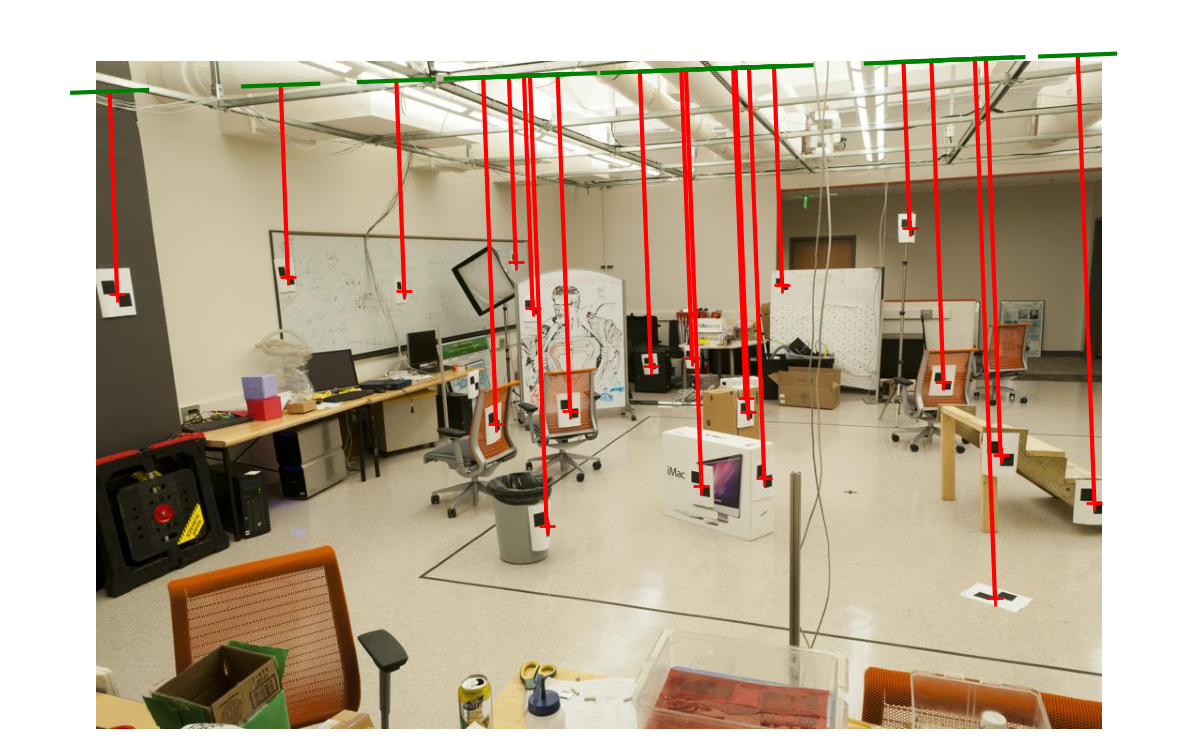
\includegraphics[width=0.45\textwidth]{./student_response/results/lab-F_unnorm.png}
	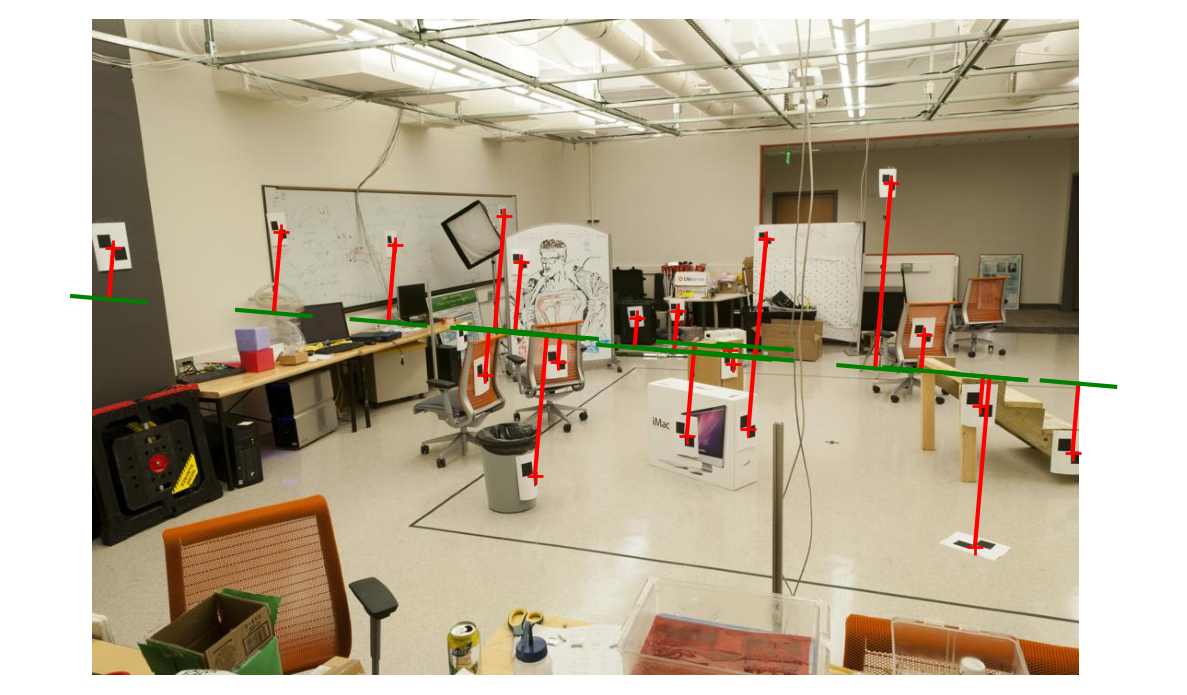
\includegraphics[width=0.45\textwidth]{./student_response/results/lab-F_norm.png}
	\caption{Fundamental matrices \( F \) (left) and \( \tilde{F} \) (right).}
\end{figure}

MSE unnorm: 125940.0390625 norm: 9330.865234375
\begin{figure}[h!]
	\centering
	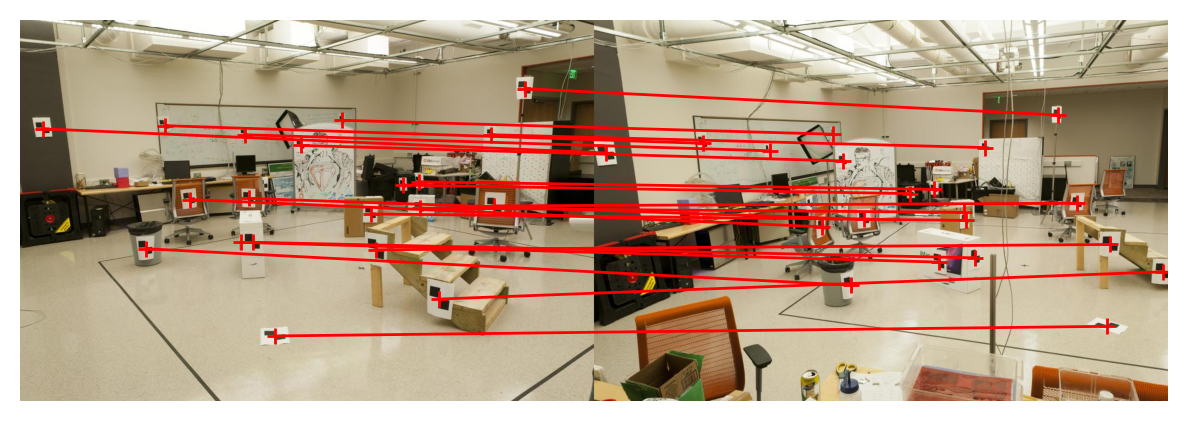
\includegraphics[width=0.45\textwidth]{./student_response/results/lab-matches.png}
	\caption{Matched keypoints}
\end{figure}

\section{Camera Calibration}

\subsection{Algorithm Description}
Camera calibration estimates the projection matrix \( P \) that maps 3D points \( X \) to their corresponding 2D points \( x \). The projection matrix is obtained by solving:
\begin{equation}
	x = P X
\end{equation}
where \( x \) is in homogeneous coordinates. The function \texttt{camera\_calibration} computes \( P \) by stacking correspondences in a matrix \( A \) and solving using SVD.

\subsection{Results}
The resulting projection matrix \( P \) for each camera is:
\begin{equation}
	P1 = \begin{bmatrix} 3.1077 * 10^{-3} & 1.3735 * 10^{-4} & -4.3170 * 10^{-4} & -9.7902 * 10^{-1} \\
		3.1395 * 10^{-4} & 6.2971 * 10^{-4} & -2.7796 * 10^{-3} & -2.0370 * 10^{-1} \\
		1.6038 * 10^{-6} & 2.8198 * 10^{-6} & -6.2774 * 10^{-7} & -1.3291 * 10^{-3} 
	 \end{bmatrix}
\end{equation}
\begin{equation}
P2 = \begin{bmatrix}
	6.9741 * 10^{-3} & -4.0607 * 10^{-3} & -1.3182 * 10^{-3} & -8.2639 * 10^{-1} \\
	1.5549 * 10^{-3} & 1.0247 * 10^{-3} & -7.3327 * 10^{-3} & -5.6298 * 10^{-1} \\
	7.7575 * 10^{-6} & 3.6385 * 10^{-6} & -1.9327 * 10^{-6} & -3.4105 * 10^{-3} 
\end{bmatrix}
\end{equation}

The MSE error between the projected 2D points and original 2D correspondences was computed using \texttt{evaluate\_points}.  
\\Image 1 MSE = 23.144485473632812
\\Image 2 MSE = 23.397932052612305

\section{Triangulation}
\subsection{Methods}
To find the 3D point \( X \) from its projections \( \mathbf{x}_1 \) and \( \mathbf{x}_2 \) in two views, we use the following projection equations:
\[
\mathbf{x}_1 \approx P_1 X
\]
\[
\mathbf{x}_2 \approx P_2 X
\]

We can enforce that \( X \) lies along the ray corresponding to each image point by taking the cross product:
\[
\mathbf{x}_1 \times (P_1 X) = 0
\]
\[
\mathbf{x}_2 \times (P_2 X) = 0
\]

This can be rewritten in terms of a skew-symmetric matrix \([ \mathbf{x}_1 \times ]\) as:
\[
[ \mathbf{x}_1 \times ] P_1 X = 0
\]
\[
[ \mathbf{x}_2 \times ] P_2 X = 0
\]

For a vector \( \mathbf{a} = [a_1, a_2, a_3]^T \), the skew-symmetric matrix \([ \mathbf{a} \times ]\) is defined as:
\[
[ \mathbf{a} \times ] = 
\begin{bmatrix}
	0 & -a_3 & a_2 \\
	a_3 & 0 & -a_1 \\
	-a_2 & a_1 & 0 
\end{bmatrix}
\]

The system of equations above can be solved using a least squares method to find the 3D point \( X \).

\subsection{Results}
The 3D reconstruction accuracy, measured as the reprojection error, is:
\begin{equation}
	\text{MSE} = 0.008938013575971127
\end{equation}

\section{Affine Factorization}

\subsection{Algorithm Description}
Using the Tomasi-Kanade factorization method, the measurement matrix \( D \) is factorized into motion matrix \( M \) and structure matrix \( S \):
\begin{equation}
	D = MS
\end{equation}
Which can be further simplified to:
\begin{equation}
	D = MQQ^{-1}S
\end{equation}
The affine ambiguity is resolved by finding matrix \( Q \) such that:
\begin{equation}
	A_i L A_i^T = I_{m \times m}
\end{equation}
where \( L = Q Q^T \). The function \texttt{get\_structure\_and\_motion} implements the factorization, and \texttt{get\_Q} finds \( Q \) via the orthogonality and equal scaling constraints.

\subsection{Results}
\\Side-by-side comparisons of \( S \) before and after eliminating affine ambiguity:
\newpage
\begin{figure}[h!]
	\centering
	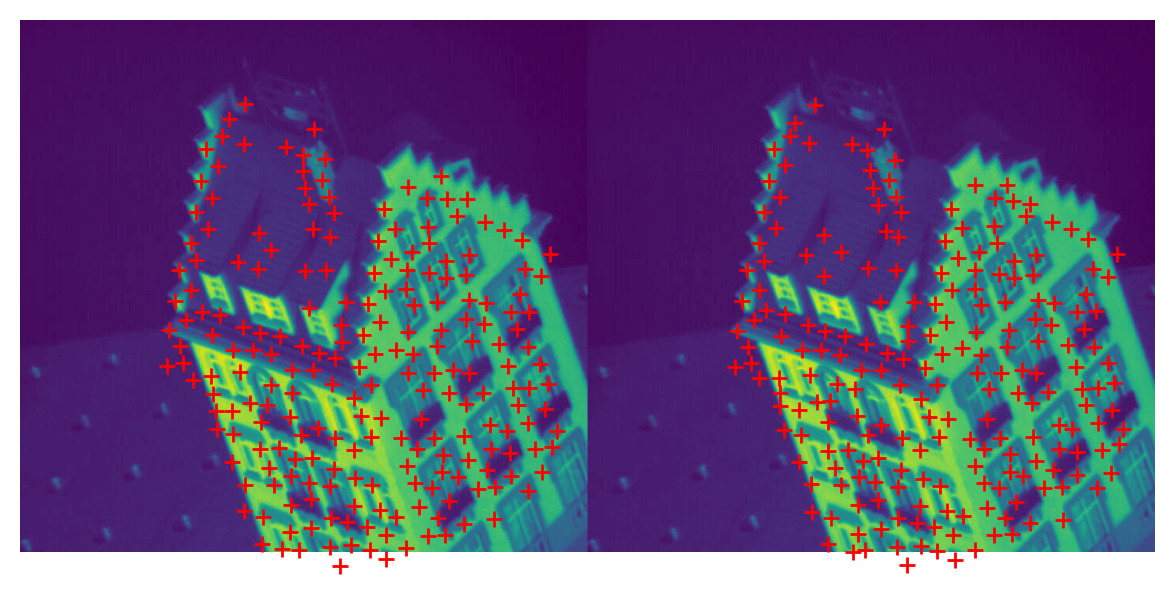
\includegraphics[width=0.45\textwidth]{./student_response/results/k00000001.png}
\end{figure}
\begin{figure}[h!]
	\centering
	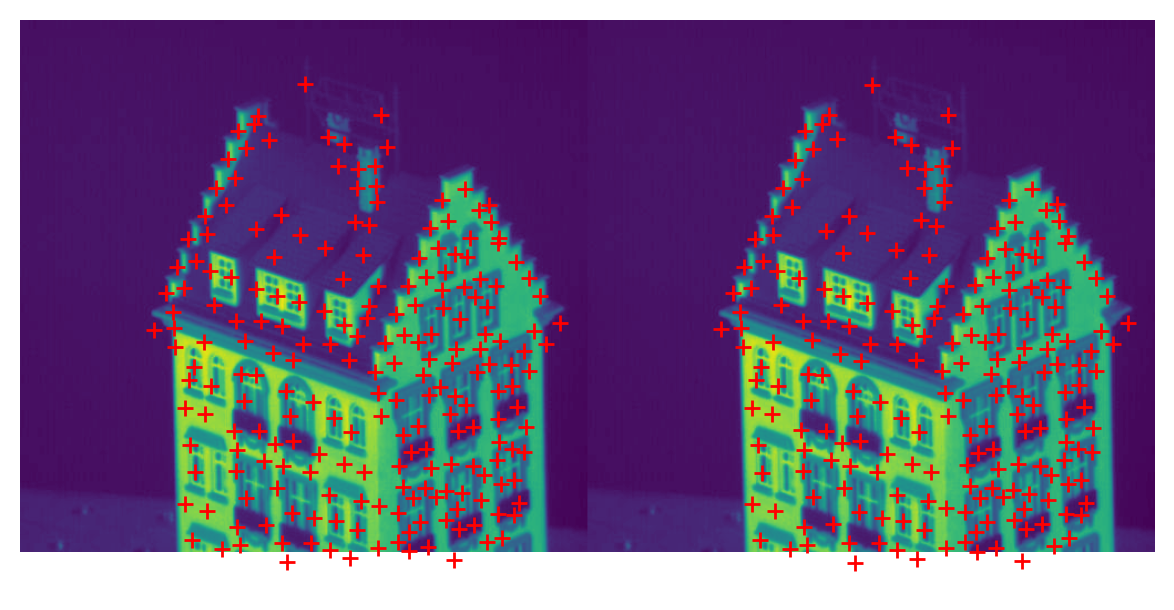
\includegraphics[width=0.45\textwidth]{./student_response/results/k00000051.png}
\end{figure}
\begin{figure}[h!]
	\centering
	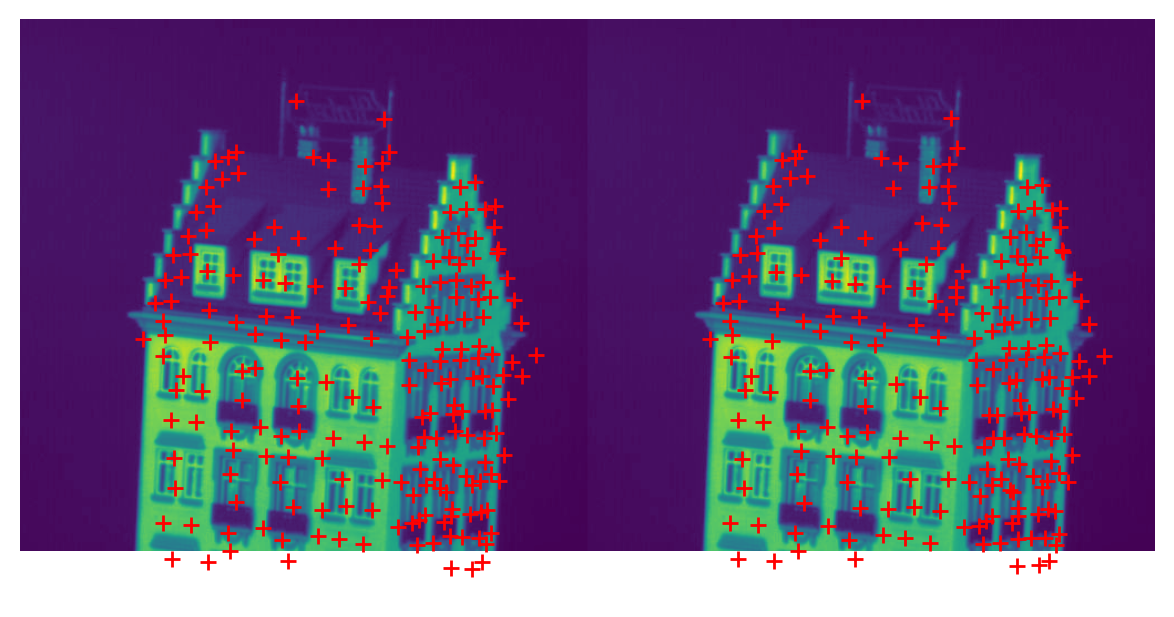
\includegraphics[width=0.45\textwidth]{./student_response/results/k00000101.png}
	\caption{Structure \( S \) before (left) and after (right) affine ambiguity elimination. These are frames 1, 51, and 101 respectively.}
\end{figure}
The MSE between observed feature points and estimated projections for selected frames is as follows:
\\Frame 1: 3.7795
\\Frame 51: 0.6229
\\Frame 101: 2.2850

\begin{figure}[h!]
	\centering
	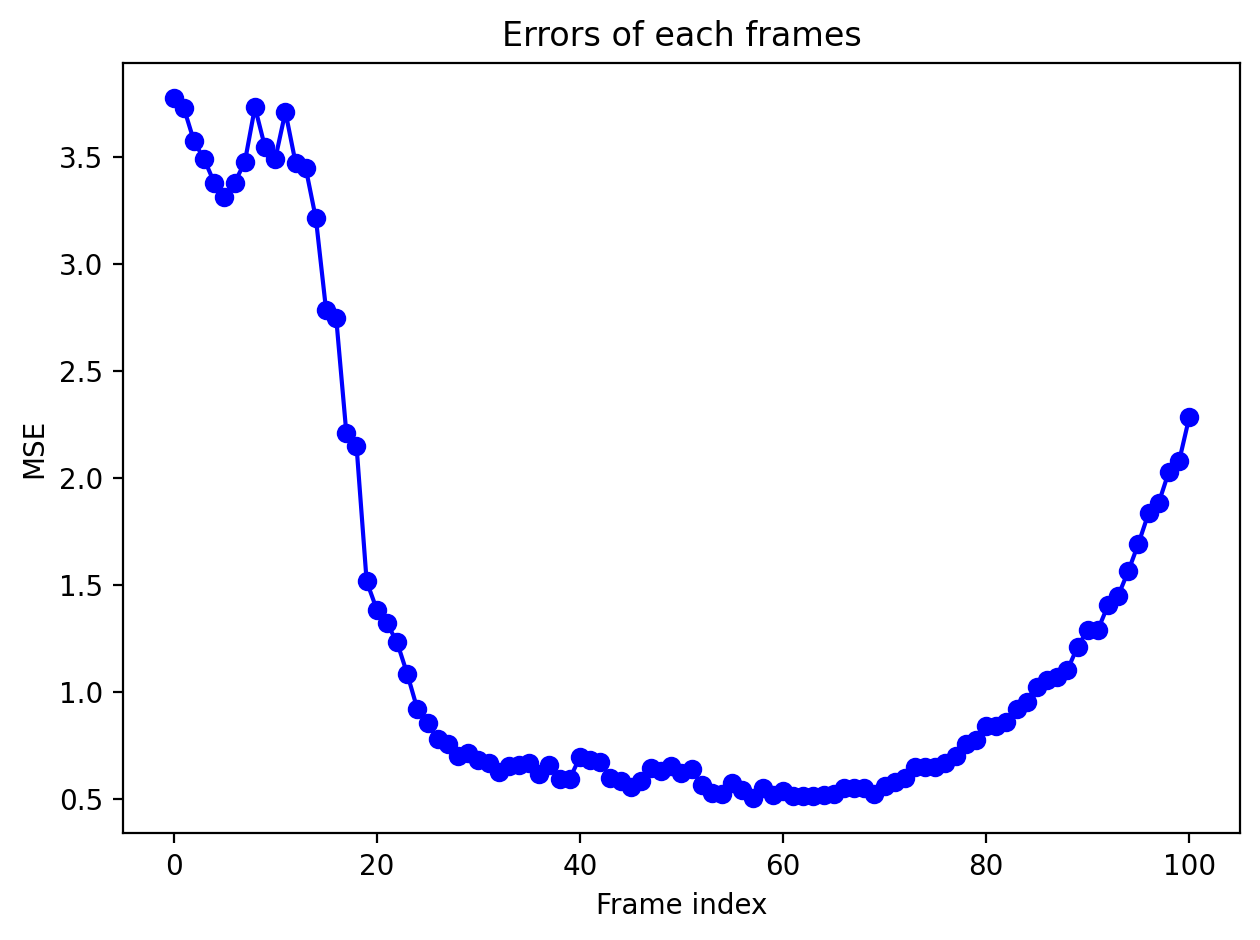
\includegraphics[width=0.45\textwidth]{./student_response/results/mse}
	\caption{MSE graph}
\end{figure}
\newpage
\section{Conclusion}
This assignment provided hands-on experience with fundamental matrix estimation, camera calibration, triangulation, and affine factorization. Through these tasks, we explored the structure-from-motion problem, examining 2D-3D correspondences and the transformation of structure and motion into a Euclidean frame.

} 